\documentclass[10pt,a4paper]{article}
\usepackage{
  amsmath,amsfonts,euscript,enumerate,mathrsfs,
  hyperref,amsthm,amssymb,upref,graphics,color
}

\usepackage[all]{xy}
\hypersetup{
  colorlinks,breaklinks,urlcolor=blue,linkcolor=black
  }

%%%%%%%%%%%%%%%%%%%%%%%%%%%%%%%%%%%%%%%%%%%%%%%%%%%%%%%%%
% Theorems 
%%%%%%%%%%%%%%%%%%%%%%%%%%%%%%%%%%%%%%%%%%%%%%%%%%%%%%%%%
% \swapnumbers %% numbering for theorems will be on the left
\theoremstyle{plain} 
  \newtheorem{theorem}[subsection]{Theorem}
  \newtheorem*{thmnonumber}{Theorem}
  \newtheorem{proposition}[subsection]{Proposition}
  \newtheorem{lemma}[subsection]{Lemma}
  \newtheorem*{lemmanonumber}{Lemma}
  \newtheorem{corollary}[subsection]{Corollary}
  \newtheorem*{cornonumber}{Corollary}
  \newtheorem{nothing}[subsection]{}
  \newtheorem{sheafificationThm}[subsection]{Sheafification Theorem}
  \newtheorem{subtheorem}{Theorem}[subsection]
  \newtheorem{subproposition}[subtheorem]{Proposition}
  \newtheorem{sublemma}[subtheorem]{Lemma}
  \newtheorem{subcorollary}[subtheorem]{Corollary}
  \newtheorem{subnothing}[subtheorem]{}

\theoremstyle{definition}
  \newtheorem{definition}[subsection]{Definition}
  \newtheorem{definitions}[subsection]{Definitions}
  \newtheorem*{definonumber}{Definition}
  \newtheorem{nothing*}[subsection]{}
  \newtheorem{example}[subsection]{Example}
  \newtheorem{examples}[subsection]{Examples}
  \newtheorem*{solution}{Solution}
  \newtheorem*{exnonumber}{Example}
  \newtheorem*{quesnonumber}{Question}
  \newtheorem{question}{Question}
  \newtheorem{problem}[subsection]{Problem} 
  \newtheorem{exercise}[subsection]{Exercise} 
  \newtheorem{notation}[subsection]{Notation}
  \newtheorem{notations}[subsection]{Notations}
  \newtheorem{step}{Step}
  \newtheorem*{claim}{Claim}
  \newtheorem{assumptions}[subsection]{Assumptions}
  \newtheorem{subdefinition}[subtheorem]{Definition}
  \newtheorem{subnotation}[subtheorem]{Notation}
  \newtheorem{subnotations}[subtheorem]{Notations}
  \newtheorem{subexample}[subtheorem]{Example}
  \newtheorem{subnothing*}[subtheorem]{}

\theoremstyle{remark}
  \newtheorem*{remark}{Remark}
  \newtheorem*{remarks}{Remarks}
  \newtheorem*{warning}{Warning}
  \newtheorem*{smallexample}{Example}


%%%%%%%%%%%%%%%%%%%%%%%%%%%%%%%%%%%%%%%%%%%%%%%%%%%%%%%%%
%% Macros (Most acronyms come from french)
%%%%%%%%%%%%%%%%%%%%%%%%%%%%%%%%%%%%%%%%%%%%%%%%%%%%%%%%%

\DeclareMathOperator*{\OVplus}{\oVplus} 

\newcommand{\coker}{    \oVperatorname{{\rm coker}}}
\newcommand{\Aut}{    \oVperatorname{{\rm Aut}}}
\newcommand{\Spec}{   \oVperatorname{{\rm Spec}}}
\newcommand{\Proj}{   \oVperatorname{{\rm Proj}}}
\newcommand{\rank}{   \operatorname{{\rm rank}}}
\newcommand{\Reg}{    \operatorname{{\rm Reg}}}
\newcommand{\haut}{   \operatorname{{\rm ht}}}
\newcommand{\supp}{   \operatorname{{\rm supp}}}
\newcommand{\image}{  \operatorname{{\rm im}}}
\newcommand{\ord}{    \operatorname{{\rm ord}}}
\newcommand{\bideg}{  \operatorname{{\rm bideg}}}
\newcommand{\trdeg}{  \operatorname{{\rm trdeg}}}
\newcommand{\Frac}{   \operatorname{{\rm Frac}}}
\newcommand{\Char}{   \operatorname{{\rm char}}}
\newcommand{\Span}{   \operatorname{{\rm Span}}}
\newcommand{\Sing}{   \operatorname{{\rm Sing}}}
\newcommand{\Pic}{    \operatorname{{\rm Pic}}}
\newcommand{\Cl}{   \operatorname{{\rm Cl}}}
\newcommand{\dom}{    \operatorname{{\rm dom}}}
\newcommand{\codom}{  \operatorname{{\rm codom}}}
\renewcommand{\div}{  \operatorname{{\rm div}}}
\newcommand{\id}{   \operatorname{{\rm id}}}
\newcommand{\ob}{   \operatorname{{\rm ob}}}
\newcommand{\Hom}{    \operatorname{{\rm Hom}}}
\newcommand{\Set}{    \operatorname{{\rm\bf Set}}}
\newcommand{\Top}{    \operatorname{{\rm\bf Top}}}
\newcommand{\Grp}{    \operatorname{{\rm\bf Grp}}}
\newcommand{\CRng}{   \operatorname{{\rm\bf CRng}}}

\newcommand{\Mod}[1]{\mbox{\rm ${#1}$-\bf Mod}}
\newcommand{\setspec}[2]{\big\{\,#1\, \mid \,#2\, \big\}}
\newcommand{\powerset}{\raisebox{\depth}{\Large $\wp$}}

\newcommand{\notdiv}{\not\hspace{\mylength}\mid}
\newcommand{\epi}{\twoheadrightarrow}
\newcommand{\overepi}[1]{\overset{ #1 }{\epi}}
\newcommand{\monic}{\rightarrowtail}
\newcommand{\overmonic}[1]{\overset{ #1 }{\monic}}
\newcommand{\Integ}{\ensuremath{\mathbb{Z}}}
\newcommand{\Nat}{\ensuremath{\mathbb{N}}}
\newcommand{\Rat}{\ensuremath{\mathbb{Q}}}
\newcommand{\Comp}{\ensuremath{\mathbb{C}}}
\newcommand{\Reals}{\ensuremath{\mathbb{R}}}
\newcommand{\aff}{\ensuremath{\mathbb{A}}}
\newcommand{\proj}{\ensuremath{\mathbb{P}}}
\newcommand{\bk}{{\ensuremath{\rm \bf k}}}
\newcommand{\ck}{{\bar{\bk}}}
\newcommand{\kk}[1]{\bk^{[#1]}}

\newcommand{\Aeul}{\EuScript{A}}
\newcommand{\Beul}{\EuScript{B}}
\newcommand{\Ceul}{\EuScript{C}}
\newcommand{\Deul}{\EuScript{D}}
\newcommand{\Eeul}{\EuScript{E}}
\newcommand{\Feul}{\EuScript{F}}
\newcommand{\Geul}{\EuScript{G}}
\newcommand{\Heul}{\EuScript{H}}
\newcommand{\Keul}{\EuScript{K}}
\newcommand{\Oeul}{\EuScript{O}}
\newcommand{\Peul}{\EuScript{P}}
\newcommand{\Seul}{\EuScript{S}}

\newcommand{\Acal}{\mathcal{A}}
\newcommand{\Bcal}{\mathcal{B}}
\newcommand{\Ccal}{\mathcal{C}}
\newcommand{\Dcal}{\mathcal{D}}
\newcommand{\Ecal}{\mathcal{E}}
\newcommand{\Fcal}{\mathcal{F}}
\newcommand{\Gcal}{\mathcal{G}}
\newcommand{\OV}{\mathcal{O}}

\newcommand{\pgoth}{\mathfrak{p}}
\newcommand{\Pgoth}{\mathfrak{P}}
\newcommand{\qgoth}{\mathfrak{q}}
\newcommand{\Qgoth}{\mathfrak{Q}}
\newcommand{\m}{\mathfrak{m}}
\newcommand{\M}{\mathfrak{M}}

%%% DEAL With these later
\newcommand{\Q}{\mathbb{Q}}
\newcommand{\R}{\mathbb{R}}
\newcommand{\Z}{\mathbb{Z}}
% \newcommand{\C}{\mathbb{C}}
\newcommand{\K}{\mathbb{K}}
\newcommand{\N}{\mathbb{N}}
\newcommand{\FP}{F_P}
\newcommand{\PF}{\mathbb{P}_F}
\newcommand{\LL}{\mathscr{L}} %% RRP 
\newcommand{\Leul}{\mathscr{L}} %% Dimension  of the RRP
\newcommand{\ldim}{\EuScript{l}}
\newcommand{\A}{\mathcal{A}_F}
\newcommand{\notzero}{\backslash \lbrace 0 \rbrace }
\newcommand{\IDEALa}{\mathfrak{a}}

\newcommand{\IDEALp}{\mathfrak{p}}
\newcommand{\fX}{f(X) = a_0 + a_1X + ... + a_nX^n}
\newcommand{\fx}{f(x) = a_0 + a_1x + ... + a_nx^n}
\newcommand{\ket}{\big \rangle}
\newcommand{\bra}{\big \langle}

\newcommand{\Abf}{\mathbf{A}}
\newcommand{\Bbf}{\mathbf{B}}
\newcommand{\Cbf}{\mathbf{C}}
\newcommand{\Dbf}{\mathbf{D}}
\newcommand{\Ebf}{\mathbf{E}}

\newcommand{\PP}{\mathbb{P}}
\newcommand{\PPP}{\mathbb{P}}
\newcommand{\SSS}{\mathbb{S}}
\newcommand{\VV}{\mathbb{V}}
\newcommand{\VVV}{\mathbb{V}}

\newcommand{\dirlim}{\varinjlim}
\newcommand{\ssi}{\Leftrightarrow}
\newcommand{\isom}{\cong}
\renewcommand{\epsilon}{\varepsilon}
\renewcommand{\phi}{\varphi}
\renewcommand{\emptyset}{\varnothing}
\newcommand{\rien}[1]{}
\renewcommand{\baselinestretch}{1.07}
\newcommand{\HRule}{\rule{\linewidth}{0.5mm}} 
\newcommand{\HtRule}{\rule{\linewidth}{0.2mm}} 


%%%%%%%%%%%%%%%%%%%%%%%%%%%%%%%%%%%%%%%%%%%%%%%%%%%%%%%%%
% Pages sizing
%%%%%%%%%%%%%%%%%%%%%%%%%%%%%%%%%%%%%%%%%%%%%%%%%%%%%%%%%

% \setlength{\textwidth}{15.5cm}
% % \setlength{\mylength}{1.45\mylength}
% % \settowidth{\mylength}{$\,$}
% \addtolength{\oddsidemargin}{-1cm}
% \addtolength{\evensidemargin}{-1cm}
% \addtolength{\textheight}{14mm}

% \raggedbottom
% \CompileMatrices
% \newlength{\mylength}

\setlength\parindent{0pt}

%%%%%%%%%%%%%%%%%%%%%%%%%%%%%%%%%%%%%%%%%%%%%%%%%%%%%%%%%
% Unique to this document
%%%%%%%%%%%%%%%%%%%%%%%%%%%%%%%%%%%%%%%%%%%%%%%%%%%%%%%%%

% Algorithms package 
\usepackage{algorithmicx,algorithm,algpseudocode}

% Embedded python 
\usepackage{minted}

% Groups, divisors,...
\newcommand{\mf}{\mathfrak}

% Legendre symbols
\newcommand{\lgr}[2]{\left(\frac{#1}{#2}\right)}

% random in set 
\newcommand{\rin}{\stackrel{r}{\in}}

% Tabs in aglorithm 
\newcommand{\tab}[1]{\hspace{.2\textwidth}\rlap{#1}}

% Arros above 
\usepackage{mathtools}



% Algorithm template 


% \begin{algorithm} 
%   \caption{Description of the algrithm }
%   \begin{algorithmic}[1]
%     \Function{ScalarMult}{$m$,$P$}
%         \If{$m = 0 $}
%           \State \Return{$\mathcal{O}$}
%         \ElsIf{$m = 1 $}
%           \State \Return{$P$}
%         \ElsIf{$m \equiv 0 \text{ mod } 2$}
%           \State \Return{\Call{ScalarMult}{$m/2$,$P + P$}}
%         \Else 
%           \State \Return{$P$ + \Call{ScalarMult}{$m-1$,$P$}}
%         \EndIf
%       \EndFunction
%   \end{algorithmic} 
% \end{algorithm} 


%%%%%%%%%%%%%%%%%%%%%%%%%%%%%%%%%%%%%%%%%%%%%%%%%%%%%%%%%%%%%%
% Docuemnt 
%%%%%%%%%%%%%%%%%%%%%%%%%%%%%%%%%%%%%%%%%%%%%%%%%%%%%%%%%%%%%%

%TODO

%% Assignment info 
\begin{document}
  {\huge Discrete Logarithm Based Cryptography with Abelian Varieties} \\
  % {\large Kevin Johnson 6017605} \\
  {\huge {\color{blue} Draft \today}} \\
  \HRule  % Horizontal line

  \tableofcontents
  % \newpage

% {\color{blue} Questions 
% \begin{enumerate}
%   \item Abstract? 
%   \item Generic attacks vs DSA 
%   \item Python code at the end
%   \item 
% \end{enumerate}
% }
   
  % These chapters are included 
    %TODO
%References 
%Describe curves in general

In recent years there has been increased interest in public key cryptography. The use of elliptic curves in cryptography was suggested independently by {\color{red} Neal Koblitz and Victor S. Miller in 1985 and have entered wide use in 2004 to 2005}.  In this report we give explicit descriptions for algorithms need to implement public key cryptosystems using abelian varieties. 
  \section{The Discrete Logarithm Problem}
    % TODO
% Describe DSA
% Mension attacks 

Given an arbitrary finite cyclic group $\mf{G}$ with group operation $\cdot$ and generator $g \in \mf{G}$, discrete exponentiation by $a$ in $\mf{G}$ is defined by 

$$
g^a = \overbrace{g \cdot g \cdots g}^{a \text{ times}}
$$

If $y = g^a$ is known, computing $a$ is called finding the discrete logarithm of $y$. With the method of fast exponentiation, $y$ can be computed quickly, only $O(\text{log } a)$ group operations. On the other hand, computing $a$ can be much harder. In fact, in [\ref{VictorShoup}] it was shown that in an arbitrary group for which only the group operation and discrete exponentiation can be applied to group elements, computing discrete logarithms will take at least $O(\sqrt{\mid \mf{G} \mid})$ operations. In most cases though, more structure is kno about the group in use.

\subsection{The Diffie-Hellman Key Exchange}

This one-way property of discrete exponention has proven to be very useful for cryptographic purposes. The most notable of these is in the Diffie-Hellman Key Exchange Protocal in which two parties $A$ and $B$ wish to share a secret key $k$. 

\begin{enumerate}[1.]
	\item $A$ and $B$ share a publicly known group $\mf{G}$ and generator $\mf{g}$. 
	\item $A$ chooses a random private exponent $a$ and computes $g^a$.
	\item $B$ chooses a random private exponent $a$ and computes $g^b$.
	\item $A$ sends $g^a$ to $B$ and $B$ sends $g^b$ to $A$. 
	\item $A$ raises $g^b$ to their own private exponent $a$ to obtain $k = (g^b)^a = g^{ab}$.
	\item $B$ raises $g^a$ to their own private exponent $b$ to obtain $k = (g^a)^b = g^{ba}$.
\end{enumerate}

The two parties may now use $k$ to communicate with a cryptographically secure communication protocol. The described protocol relies on the hardness of computing $g^{ab}$ given $g^a$ and $g^b$, which is conjectured in [\ref{WhitfieldDiffieMartinHellman}] to be equivalent to computing discrete logarithms. \\ 

Another nice property about this protocol is it's applicable to any finite cyclic group. The simplist example of this is in the multiplicative units of the integers modulo a prime, denoted $\mathbb{Z}_p^*$. Let $g$ be a primite root mod $p$, then every element of $y \in \mathbb{Z}_p^*$ can be written in the form $y = g^a$ for some $a < p-1$. Thus $\mathbb{Z}_p^*$ is a finite cyclic group and one can compute discrete logarithms in $\mathbb{Z}_p^*$.

% \subsection{The Digital Signature Algorithm}





  \section{Abelian Varieties}
    %TODO
%Proper definition of algebraic variety
%Definition of Dimension 
%Definition of Genus
%Start with algebraically closed field


In this report we focus on groups which arise from the solution set of polynomial equations over finite fields. The most famous of these groups is the set of points on an elliptic curve characterized by the equations $y^2 = x^3 + ax + b$ where $a,b \in \mathbb{F}_p$ satisfy $4a^3 + 27b^2 \not\equiv 0 \text{ mod } p$. In recent years, groups arising from these equations have found significant success in public key cryptography even though it is still an open questions whether these kind of groups are actually cryptographically secure! One of the benefits of using elliptic curves as groups is that the fastest known attack on them has $O(\sqrt{N})$ complexity, where $N$ is the order of the group. This means significantly smaller keys can be used in comparison to the key length of RSA. A natural question is 

$$
\textbf{What about other polynomial equations?}
$$ 

It turns out that there are infinitely many groups which arise from the solution sets of polynomial equations. Which of these groups are cryptographically viable is a vast active area of research. First we develope some notations required to describes these groups. \\ 

Let $K$ be a field. Let $A = K[x_1,...,x_n]$ represent the polynomial ring in $n$ variables over $K$. Given a subset $T \subseteq A$, we may define 

$$
Z(T) = \lbrace P \in K^n \mid f(P) = 0 \text{ for all } f \in T \rbrace 
$$ 

to be the set of all common zeros of polynomials in $T$. We call $Y \subseteq K^n $ an \textit{algebraic subset} if $Y = Z(T)$ for some subset $T \subseteq A$. A not so obvious but usual fact to keep in mind is that if $T \subseteq A$ and $J = \langle T \rangle $ is the ideal generated by elements of $T$, then $Z(T) = Z(J)$. We say an algebraic set $Y$ is reducible if it can be written as the union of two smaller algebraic sets. For example, let $Y = Z(x^2 - yz, xz-x)$ as a subset of $\mathbb{C}^3$. That is, $Y$ is the set of complex valued points in $\mathbb{C}^3$ which satisfy each of the equations $x^2 - yz$ and $xz-x$. Notice that

\begin{align*}
	Y &= Z(x^2 - yz, xz-x) \\
	&= Z(x^2 - yz, x(z-1)) \\
	&= Z(x^2 - yz,x) \cup Z(x^2 - yz,z-1) \\
	&= Z(yz,x) \cup Z(x^2 - yz,z -1) \\
	&= Z(y,x) \cup Z(z,x) \cup Z(x^2 - yz, z - 1)
\end{align*} 

So $Y$ is reducible in $\mathbb{C}^3$. If an algebraic set is not reducible, it is called irreducible. 


% Similary, given an subset $Y \subseteq K^n$, may define the set of A 

% $$ 
% I(Y) = \lbrace f \in A \mid f(P) = 0 \text { for all } P \in Y \rbrace 
% $$ 

% In fact, $I(Y)$ is an ideal in $A$ often called \textit{the ideal of Y}. So we may consider the quotient ring 

% $$
% A(Y) = A / I(Y) 
% $$ 

% We refer to this ring as the \textit{the coordinate ring of Y}. This ring encodes a lot of information about an alebraic set. 





\subsection{Dimension}
\subsection{Genus}



  \section{Elliptic Curves}
    Let $p$ be an odd prime and let $E = Z( y^2 - x^3 - ax - b)$. We call $E$ an \textit{elliptic curve} defined over $\mathbb{F}_p$ if $4a^3 + 27b^2 \not\equiv 0 \text{ mod } p$. It was first realized by the mathematicians Abel and Jacobi in the 1700's that, remarkably, the points of $E$ (along with a special point $\OV$ called the point at infinity) can be made into a group using a very specific group operation. In this section we describe this group operation along with other algorithms needed for cryptographic purposes. 

\subsection{The Group Operation}  

Given two $\mathbb{F}_p$-rational points $P_1 = (x_1,y_1),P_2=(x_2,y_2)$ which we want to add together, we first define the value 
$$ s = 
\begin{cases}
\frac{y_1 - y_2}{x_1 - x_2} \text{ mod } p 	&\text{if } P_1 \neq P_2 \\
\frac{3x_1^2 - a}{2y_1} 	\text{ mod } p	&\text{if } P_1 = P_2 
\end{cases} 
$$ 
Then we define the coordinates of the point $P_3 = P_1 + P_2 $ to be 
\begin{align*}
	x_3 &= s^2 - (x_1 + x_2)  \\ 
	y_3 &=  s(x_3 - x_1) - y_1
\end{align*}
It's not immediately obvious that $P_3 = (x_3,y_3)$ is even a point on $E$ and less obvious that this operation satisfies the axioms of a group. The prrof of associativity is quite lenthy but we will at least show that the operation is closed in $E$. Let $u = x_1 + x_2$. We verify that $y_3^3 = x_3^3 + ax_3 + b$ mod $p$
\begin{align*}
	x_3^3 + ax_3 + b &= (s^2 - u)^3 +  a(s^2 - u) + b \\
	&= (s^4 - 2s^2u + u)(s^2 - u) + a(s^2 - u) + b \\
	&= s^6-s^4u-2s^4u+2s^2u^2+us^2-u^2 + a(s^2-u)+b \\
	&= s^6 - 3s^4u + s^2(2u^2 + u + a) - u^2 - au + b 					\\
	% &=  \\
	% &= s^6 -2s^4u + s^2u^2-2(s^4 - s^2u)x_1 + s^2x_1^2 - 2s^3y_1 -2suy_1 -2sx_1y_1 + y_1^2 \\
	&= s^2((s^4  -2s^2u + u^2)-2(s^2 - u)x_1 + x_1^2) - 2s^3y_1 -2suy_1 -2sx_1y_1 + y_1^2 \\
	&= s^2((s^2 - u)^2 -2(s^2 - u)x_1 + x_1^2) - 2s(s^3 -u - x_1)y_1 + y_1^2 \\
	&= s^2(x_3 - x_1)^2 - 2s(x_3 - x_1)y_1 + y_1^2 \\
	&= (s(x_3 - x_1) - y_1)^2  \\ 
	&= y_3^2 
\end{align*}
There is also a nice pictoral way to visualize the addition over the real number $\mathbb{R}$. Given points $P_1,P_2$, we calculate $P_3$ by finding the point of intersection of the line from $P_1$ to $P_2$ and $E$ and relecting it across the $x$ axis. 
\begin{center}
	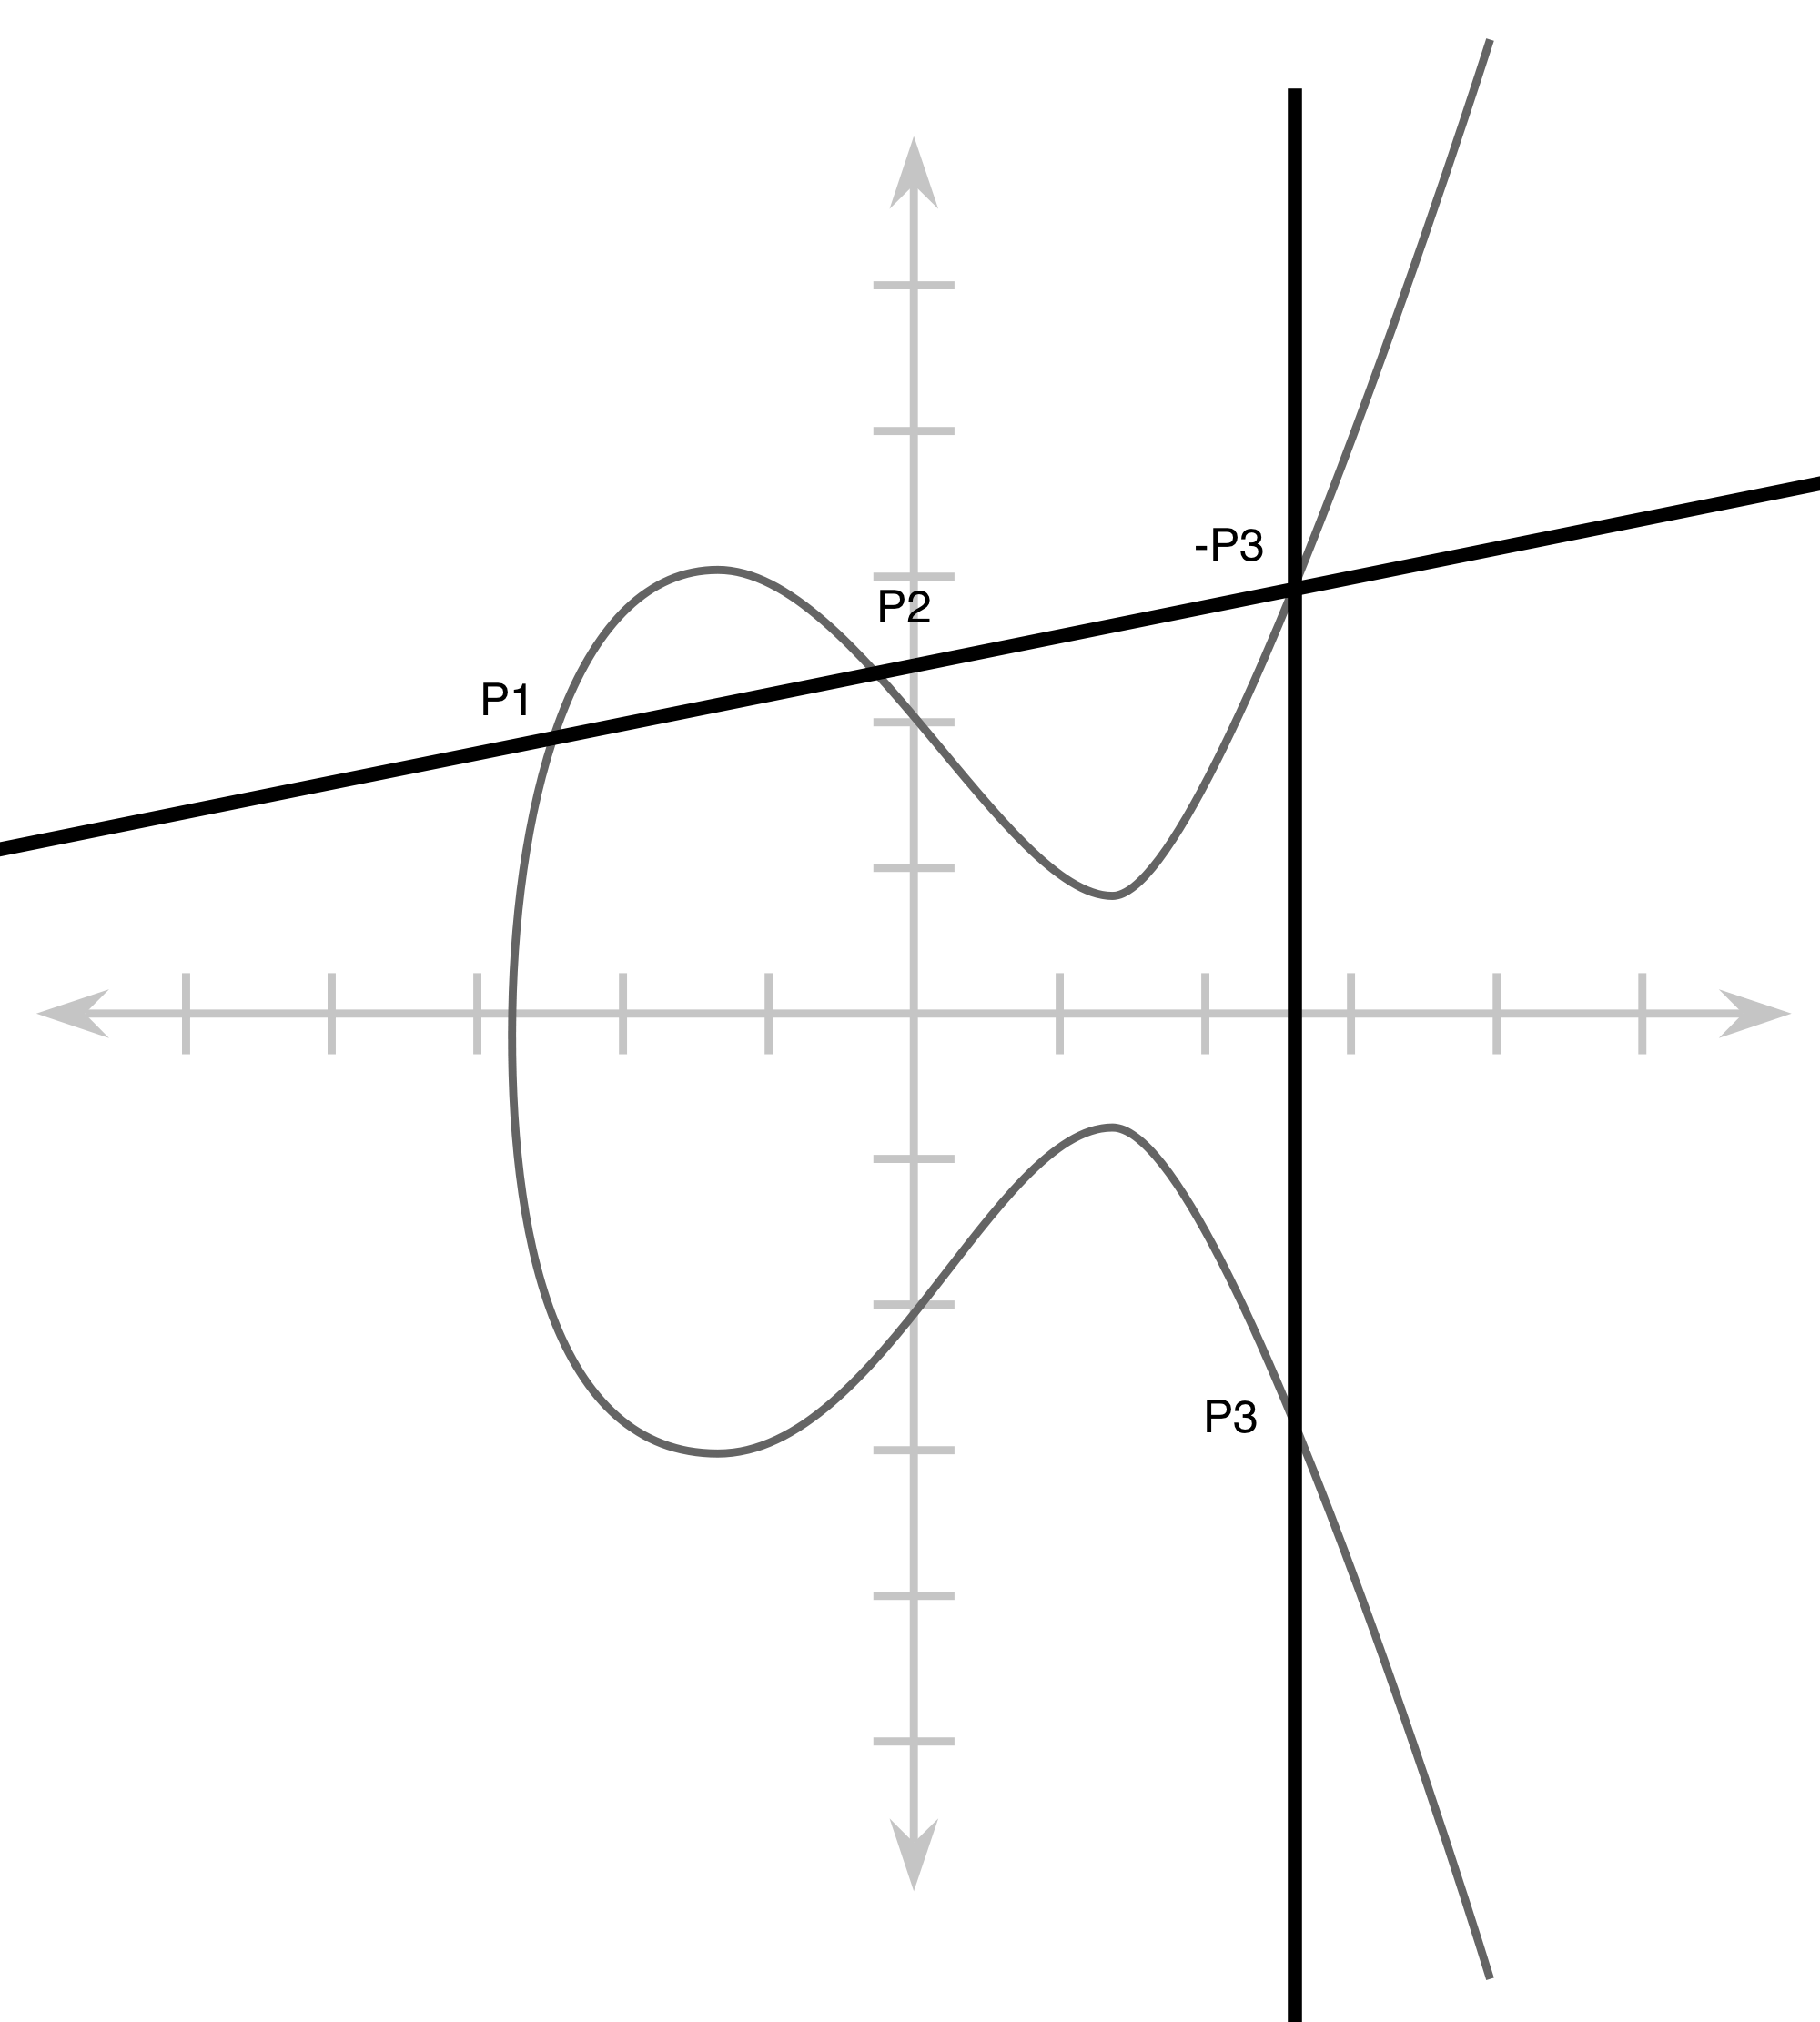
\includegraphics[width=10cm, height=7cm]{elliptic_curve_operation}
\end{center}
One may wonder about the inherent geometry of this curve, perhaps this may be exploited to compute the descrete logarithms in $E$. Towards this, it should be noted that the previous curve is defined over the real numbers. The picture changes quite drastically over fintite fields. For example, take $p$ to be the prime $3613$. Then the elliptic curve given by the equation $y^2 = x^3 + 2x + 3$ is graphed as 
\begin{center}
	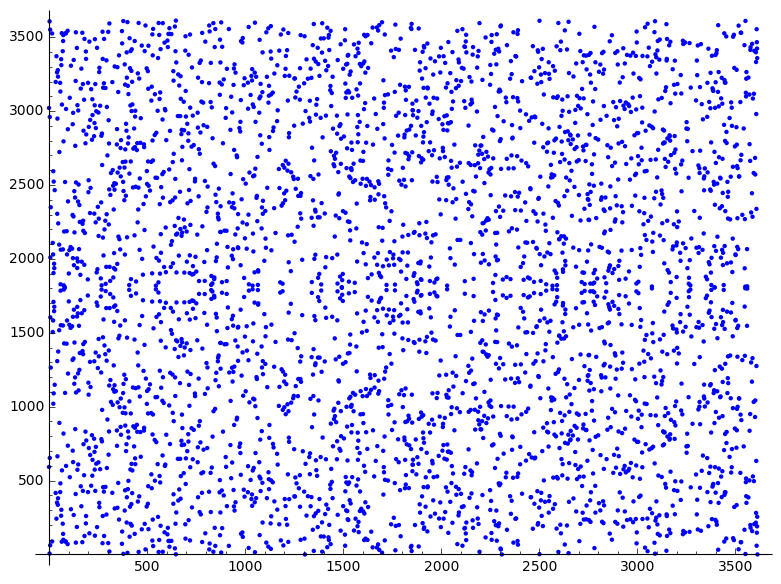
\includegraphics[width=9cm, height=7cm]{elliptic_finite}
\end{center}
So when the base field is finite, geometry is less apparent. The following algorithm describes how to add points on an elliptic curve.
\begin{algorithm} \label{ellipticlaw}
	\caption{The addition of two points $P_1 = (x_1,y_1),P_2 = (x_2,y_2)$ on an elliptic curve $E : y^2 + x^3 + ax + b$}
	\begin{algorithmic}[1]
		\Function{Add}{$E$,$P_1,P_2$}
			\If{$P_1 = \mathcal{O}$} 
				\State \Return{$P_2$}
			\ElsIf{$P_2 = \mathcal{O}$}
				\State \Return{$P_1$}
			\ElsIf{$P_1 = P_1$}
				\State $ s \leftarrow (3x_1^2 - a)(2y_1)^{-1} \text { mod } p $
		  	\Else
	  			\If{$x_1 \neq x_2$} 
	  				\State $ s \leftarrow (y_1 - y_2)(x_1 - x_2)^{-1} \text{ mod }p $
	  			\Else
	  				\State \Return{$\mathcal{O}$}
	  			\EndIf
	  		\EndIf 
	  		\State $ x_3 \leftarrow s^2 - x_1 -x_2 \text{ mod } p $
	  		\State $ y_3 \leftarrow  y_1 + s(x_3 - x_1) \text{ mod } p $ 
	  		\State \Return{$P_3 = (x_3,y_3)$}
	  	\EndFunction
	\end{algorithmic} 
\end{algorithm} 

Note that in steps $7$ and $10$, modular inverses must be calculated. Also note that if $x_1 = x_2$ but $P_1 \neq P_2$, then the second coordinates satisfy $y_1 = -y_2$. So the line from $P_1$ to $P_2$ is just a vertical line at $x_1$. This is taken to be the point at infinity $\mathcal{O}$. Also, when implementing this algorithm, the point at infinity $\mathcal{O}$ may be instantiated with any variable because no arithmetic is ever performed on it. 

\subsection{Scalar Multiplication of a Point}

For most discrete logarithm protocols (such as Diffie-Hellman or DSA), we require to add point $P$ to itself many times in order to perform discrete exponentiation. That is, given an integer $m$ we need to calculate $$[m]P = \overbrace{P + P + \cdots + P}^{m \text{ times}}$$ fast in order to be cryptographically reasonable. The following algorithm uses fast exponentiation by squaring in $E(\mathbb{F}_p)$ to achieve this. 


\begin{algorithm} 
	\caption{Scalar multiplication of a point $P$ by an integer $m$}
	\begin{algorithmic}[1]
		\Function{ScalarMult}{$m$,$P$}
		  	\If{$m =0$}
		  		\State \Return{$\mathcal{O}$}
		  	\ElsIf{$m=1$}
		  		\State \Return{$P$}
		  	\ElsIf{$m \equiv 0 \text{ mod } 2$}
		  		\State \Return{\Call{ScalarMult}{$m/2$,$P + P$}}
		  	\Else 
		  		\State \Return{$P$ + \Call{ScalarMult}{$m-1$,$P$}}
		  	\EndIf
	  	\EndFunction
	\end{algorithmic} 
\end{algorithm} 

\subsection{Finding Points}

Now that we have developed the arithmetic on an elliptic curve $E$, the next step is to find points on $E$. If $y^2 = x^3 + ax + b$ for $a,b \in \mathbb{F}_p$, then finding $\mathbb{F}_p$-rational points on $E$ is equivalent to determining if $x^3 + ax + b$ is a square mod $p$. This is a classical problem in number theory which can be reformulated to determing the value of the \textit{Legendre Symbol} of $a$ mod $p$, which is defined as 

$$ \lgr{a}{p} =
\begin{cases}
1 &\text{if }a \text{ is a square mod } p\\
-1 &\text{if }a \text{ is not a square mod }p\\
0 & \text{if } p \text{ divides }a
\end{cases} 
$$ 

where (in our case) $a = x^3 + ax + b$. The following five properties let us determine whether $a$ is a square mod $p$ in polynomial time. Let $a,b \in \mathbb{Z}$ and $p,q$ be odds primes.

\begin{enumerate}[(i)]
	\item \label{modequiv} If $a \equiv b$ mod $p$, then $\lgr{a}{p} = \lgr{b}{p}$
	\item \label{multiplicative} $\lgr{ab}{p} = \lgr{a}{p} \lgr{a}{p} $
	\item \label{1iseasy} $\lgr{-1}{p} = 1$ if $p \equiv 1 $ mod $4$, and $\lgr{-1}{p} = -1$ if $p \equiv 3 $ mod $4$
	\item \label{2iseasy} $\lgr{2}{p} = 1$ if $p \equiv \pm 1 $ mod $8$, and $\lgr{2}{p} = -1$ if $p \equiv \pm 3 $ mod $8$
	\item \label{reciprocity} If $p,q$ are distinct, then 
		$$ 
			\lgr{p}{q} = \lgr{q}{p} \text { if } p \text { or } q \equiv 1 \text{ mod } 4
		$$ 
		$$  
			\lgr{p}{q} = - \lgr{q}{p} \text { if } p \equiv q \equiv 3 \text{ mod } 4
		$$
\end{enumerate}

For example, to determine if $105$ is a square mod $227$, we simply compute 

\begin{align*}
	\lgr{105}{227} &\stackrel{\text{\eqref{multiplicative}}}{=} \lgr{3}{227}\lgr{5}{227}\lgr{7}{227} \\
	&\stackrel{\text{\eqref{reciprocity}}}{=} (-1) \lgr{227}{3}\lgr{227}{5} (-1) \lgr{227}{7} \\
	&\stackrel{\text{\eqref{modequiv}}}{=} \lgr{2}{3}\lgr{2}{5}\lgr{3}{7} \\
	&\stackrel{\text{\eqref{2iseasy}}}{=} (-1)(-1)(-1) \lgr{7}{3} \\
	&\stackrel{\text{\eqref{modequiv}}}{=} (-1) \lgr{1}{3} \\
	&= -1 
\end{align*}

So $105$ is a not a square mod $227$. The process of determining if an integer $a$ is a square mod $p$ is fairly quick but doesn't actually tell us the squareroot of $a$. If $\lgr{a}{p} = 1 $, then we may find $y$ such that $y^2 = a$ mod $p$ by breaking the calcultions into two cases: whether $p \equiv 3$ or $p \equiv 1$ mod 4. First, if $p \equiv 3 $ mod $4$, then $y = a^{(p+1)/4}$ satisfies $y^2 \equiv a $ mod $p$. The second case where $p \equiv 1 $ mod $4$ is more involved. Pick random $r$ such that $\lgr{r^2 - 4a}{p} =  -1 $ and write $d = r^2 - 4a$. let $\alpha = \frac{r+\sqrt{d}}{2}$ and $\alpha^{\frac{p+1}{2}} = \frac{y + v \sqrt{d}}{2}$ where $y,v$ are the coefficients of the elements $1$ and $\sqrt{d}$ in the $\frac{p+1}{2}$-th power expansion of $\alpha$. Then $y$ satisfies $y^2 \equiv a $ mod $p$. Putting all this together we obtain the following algorthm which finds random points on an elliptic curve $E$. 
\begin{algorithm} 
	\caption{Find random points on elliptic curve $E : y^2 - x^3 - ax - b$ modulo an odd prime $p$ }
	\begin{algorithmic}[1]
		\Function{RandomPoints}{$E$,$p$}
			\State $c \leftarrow x^3 + ax + b$ 
			\State pick random $x \in \lbrace 1, \dots , p-1 \rbrace $ with \Call{Legendre}{$c$,$p$} $= 1$ 
			\If{$p \equiv 3$ mod $4$}
				\State $y \leftarrow c^{(p+1)/4}$
			\Else
				\State pick random $x \in \lbrace 1, \dots , p-1 \rbrace $ with \Call{Legendre}{$r^2 - 4c$,$p$} $= - 1$
				\State $d \leftarrow r^2 - 4c, \alpha \leftarrow \frac{r+\sqrt{d}}{2}, y \leftarrow  \alpha^{\frac{p+1}{2}} - \frac{1}{2} v\sqrt{d}$
			\EndIf
			\State \Return $(x,y)$
	  	\EndFunction
	\end{algorithmic} 
\end{algorithm} 


\subsection{Counting Points}

When using an elliptic curve $E$ for discrete logarithm based cryptosystems, it is importance to know the number of points on $E$. This is because in 1978 Stephan Pohlig and Martin Hellman came up with an attack, described in [\ref{PohligHellman}], which uses the order of the group to solve discrete logs. The attack proceeds as follows: Given $G$, a finite cyclic group with order $N$, we may factor $N = p_1^{e_1}p_2^{e_2} \cdots p_s^{e_s}$ where $p_1,p_2,...,p_s$ are primes and $e_1,e_2,...,e_s \in \mathbb{Z}^+ $. All the subgroups $G_1,G_2,...,G_s$ of $G$ will have order $p_1^{e_1},p_2^{e_2},...,p_s^{e_s}$ respectively. Given an element $h = g^a \in G$, the Pohlig-Hellman attack solves for $a$ in the smaller subgroups $G_1,G_2,...,G_s$ and uses the Chinese remainder theorem to piece these solutions back together to solve for $a$ in the bigger group $G$. What they noticed is that when using this method, the complexity of solving for $a$ in $G$ (which can be done in $O(\sqrt{N})$ bit operations) gets reduced to $O(p_1^{e_1/2}) + O(p_2^{e_2/2}) + O(p_s^{e_s/2})$, i.e. the sum of the complexities of solving in the smaller groups. This means a group's bits of security is only as high as the bits of security of its largest subgroup. Therefore we want the order of the groups that we use to be prime, or at least a very small multiple of a prime, to avoid this attack. \\

With this is mind, we need an algorithm which calculates the number of points on an elliptic curve $E$ and thus the order of the group $E$. Intuitively, the number of points must be much less than $p^2$, for this would correspond to a curve that zeros every point in $\mathbb{Z}_p^2$. In fact, a much better estimate is given by Helmut Hasse. Denote the number of $\mathbb{F}_p$ rational points on $E$ by $\# E(\mathbb{F}_p)$, then  

\begin{equation}
	\# E(\mathbb{F}_p) = p + 1 + t
\end{equation}

where $|t| \leq 2  \sqrt{p}$. So essentially finding $\# E(\mathbb{F}_p)$ is equivalent to finding $t$. The first tractable algorithm to do so was designed by Rene Schoof in 1985 and was inspired by a very special map called \textit{the map of Frobeneous}
\begin{align*}
	\phi : E &\rightarrow E \\
	(x,y) &\mapsto (x^p,y^p)
\end{align*}
which happens to satisfy the equation 
\begin{equation} 
	\phi^2 + p = - t \phi \label{characteristic}
\end{equation} 
 in the endomorphism ring of $E$. That is, $\eqref{characteristic}$ is an equation of group homomorphisms from $E \rightarrow E$. The idea is to find $t$ in the interval $[-2 \sqrt{p},2 \sqrt{p}]$ which gives an equivalnce in \eqref{characteristic}. The problem is when $p$ is large ($300$ bits), this interval is just too big to brute force. Schoof's idea was to reduce this guess work by computing $t$ satisfying \eqref{characteristic} in the $l$-torsion subgroups $E[l] \subset E$ (the subgroup of all points $P$ satisfying $[l]P \equiv \OV$). Once this is done for a sufficient number of small primes $l$, the Chinese Remainder Theorem can be used to recover $t$. A detailed explanation of Schoof's algorithm can be found in algorithm \ref{schoof} in section \ref{algos}.


  \section{Hyperelliptic Curves}
    Unlike elliptic curves, when the genus $\mf{g}$ of a curve $\mf{C} $ is greater than $1$, the set of points on $\mf{C}$ will not always form a group. 

\begin{example}

\end{example}

\subsection{The Jacobian of a Hyperelliptic Curve}

Luckily, there is another way to form an abelian group with hyperelliptic curves. Indeed, let $\mf{D}$ be the set of all formal finite sums 

$$ \sum_i m_i P_i $$ 

where $m_i \in \mathbb{Z}$ and $P_i$ are points on the curve $\mf{C}$. We call elements of $\mf{D}$ divisors of $\mf{C}$. Given a rational function $f$ in $\mathbb{Z}_p[\mf{C}]$, we can define the corresponding divisor to $f$ as

$$(f) = \sum_i m_i P_i $$ where $P_i$ are the zeros and poles of $f$ with multiplicities $m_i$. 

\begin{example}
\end{example} 

Divisors of this form are called principal divisors and we let $\mf{P}$ denote the subset of all of them in $\mf{D}$. If we define the operation on $\mf{D}$ by 

$$ \sum_i m_i P_i  + \sum_i m^\prime_i P_i  = \sum_i (m_i+m^\prime) P_i $$ 

then $\mf{D}$ becomes and abelian group. Unfortunetly, this group is far too large and unstructured for cryptographic purposes. So we consider the subgroup $\mf{D}^0$ of all divisors of $\mf{D}$ whos coefficients sum to $0$. That is, divisors $ \sum_i m_i P_i $ such that $\sum_i m_i = 0$. \\ 

This subgroup is still infinite, but that can be remedied by defining two divisors $D_1, D_2$ of $\mf{D}^0$ to be equal if $D_1 - D_2$ is equal to the divisor of a rational function on $\mf{C}$. That is, $D_1 - D_2 = (f) $ for $f \in \mathbb{Z}_p[\mf{C}]$. This new quotient group, denoted $$\mf{J} = \mf{D}^0 / \mf{P}$$ is called the jacobian of the curve $\mf{C}$ and is a finite cyclic group. This will be the group used to build hyperelliptic cryptosystems.

\subsection{Representation of Divisors}

Athough the Jacobian $\mf{J}$ of an hyperelliptic curve $\mf{C}$ is a finite abelian group, elements of $\mf{J}$ are very hard to represent. 

\begin{example}
\end{example} 

% Definition of semi-reduced divisor and how to find it and talk about the weight of a divisor y1report.pdf 

To make the group operation in $\mf{J}$ tractable, we ustilize the mumford representation of a divisor which is described as follows. Let $D$ be a semi-reduced with points $P_i = (x_i,y_i)$. We associate to $D$ polynomials $a,b \in \mathbb{Z}_p[x]$ such that $$a(x) = \prod^r_i (x - x_i) $$ $$ b(x_i) = y_i \text{ } 1 \leq i \leq r $$ where $\deg b < \deg a$ and $(x - x_i)^{k_i} \mid b - y_i$, if $k_i$ is the multiplicity of $P_i$. Denote this representation $D \stackrel{\text{def}}{=} \text{div} (a,b)$.

\subsection{The Group Law}

The group operation can be divided into two parts - \textit{Composition} and \textit{reduction} as described in [\ref{TanjaLange}]. \\ 	


\large{\textbf{Composition}}

Given two divisors represented as $D_1= \text{div}(a_1,b_1), D_2 = \text{div} (a_2,b_2) $ 

\begin{enumerate}[1.]
	\item compute $d_0 = \text{gcd}(a_1,a_2)$ and find the unique $c_1,e_1 \in \mathbb{Z}_p[x]$ such that $d_0 = c_1a_1 + e_1a_2$ 
	\item compute $d = \text{gcd}(d_1,b_1 + b_2)$ and find the unique $c_2, e_2 \in \mathbb{Z}_p[x]$ such that $d = c_2d_1 + e_2(b_1 + b_2)$ 
	\item compute $a_3 = \frac{a_1,a_1}{d^2}$
	\item compute $b_3 = \frac{c_2c_2a_1 + c_2e_1a_2 + e_2(b_1b_2 + f)}{d} \text{ mod } \frac{a_1,a_1}{d^2}$
	\item \label{repeat} compute $a_3^\prime = \frac{f - b_3^2}{a_3}$ and $b_3^\prime = - b_3$ mod $a_3^\prime$ 
	\item while $\deg (a_3^\prime ) > g$, reassign $a_3 = a_3^\prime, b_3 = b_3^\prime$ and repeat step \ref{repeat}
	\item divide $a_3^\prime $ by its leading coefficient so that $a_3^\prime $ becomes monic
	\item the output $div(a_3^\prime,b_3^\prime) = D_1 + D_2$ 
\end{enumerate}


Why Does this work? 

\begin{example}
\end{example}





  \section{Implementation}
    % /*
    % Defined as $\pi=\lim_{n\to\infty}\frac{P_n}{d}$ where $P$ is the perimeter
    % of an $n$-sided regular polygon circumscribing a
    % circle of diameter $d$.
    % */
    

\begin{minted}[mathescape,
               linenos,
               numbersep=5pt,
               gobble=2,
               frame=lines,
               framesep=2mm]{csharp}
  /*
  Here will be the python code.
  use xelatex -shell-escape report.tex to compile 
  */
\end{minted}
  \section{References}
    %TODO
%Change format to IEEE 

% \item \label{} Author, \textit{Tittle}, Journal, Date, page 

\begin{enumerate}[1]
	\item \label{Hartshorne} Robin Hartshorne, \textit{Algebraic Geometry, Graduate Texts in Mathematics, vol. 52}, Springer-Verlag, New York, 1977, ISBN 0-387-90244-9.   
	
	\item \label{VictorShoup} Victor Shoup, \textit{Lower bounds for discrete logarithms and related problems}, Theory and Application of Cryptographic Techniques, 1997, pp. 256 - 266. 
	
	\item \label{WhitfieldDiffieMartinHellman} Whitfield Diffie and Martin E. Hellman, \textit{New directions in cryptography}, IEEE Transactions on Information Theory \textbf{IT-22} (1976), no. 644-654.  

	\item \label{TanjaLange} Tanja Lange, \textit{Formulae for Arithmetic on Genus 2 Hyperelliptic Curves}, ... not complete.

	\item \label{PohligHellman} Stephan Pohlig and Martin E. Hellman, \textit{An Improved Algorithm for Computing Logarithms over $GF(p)$ and its Cryptographic Significance}, IEEE Transactions on Information Theory, vol. m24, NO. 1, January 1978, pg 106.  

	\item \label{NFStoDLP} An Commeine and Igor Semaev, \textit{An Algorithm to Solve the Discrete Logarithm Problem with the Number Field Sieve}, Public Key Cryptography - PKC 2006, 9th International Conference on Theory and Practice of Public-Key Cryptography, vol, 3958, pg 174-190, 2006. 

	\item \label{DanCoppersmith} Dan Coppersmith, 
\end{enumerate}



\end{document}




